% TODO:
% Please mark yourself here and push
% if you are in progress on something!

% - RB tree conclusion
% - Real-world problem solving

% - RB trees practical implementation   <- Darrin
% - RB trees real-world application
% - RB tree theory question 2			<- Logan
% - RB tree comparative analysis

% - Maxflow theory question 2           <- Jordan
% - Maxflow real-world application      <- Kate

\documentclass[12pt]{amsart}

\usepackage[margin=0.75in]{geometry}
\usepackage{amssymb}
\usepackage{amsmath}

% Image setup
\usepackage{graphicx}
\graphicspath{{./images/}}

\title{Exploration and Analysis of Red-Black Trees and Max Flow
    Algorithms}
\author{Jordan Dehmel, Kate Eckhart, Logan Humbert, Darrin Miller}
\date{December 4th, 2023}

\begin{document}

\maketitle

\tableofcontents

\section{Abstract}

    We explore various properties and real-world applications of
    red-black trees and max-flow optimization algorithms. We
    explore several algorithms for the later, and provide
    experimental comparative analysis of their performances.

\newpage
\section{Introduction}

\subsection{Efficient Tree-Based Lookup Structures}

    The Binary Search Tree (BST) is a vital data structure for
    efficient lookups in large lookup tables. However, they have
    their issues. While a BST can provide lookups in logarithmic
    time in the best-case scenario, this can quickly devolve
    into linear time given suboptimal insertion order. For
    instance, if data is inserted into a BST in monotonically
    ascending order, each node in the tree will have only right
    children. This quickly devolves into linear lookup time!
    This weakness motivates the need for a tree data structure
    which can be proven to avoid this worst-case scenario.

    Several such tree-based data structures exist; The 2-3-4
    tree and the red-black tree. Both of these structures can
    be proven to remain perfectly balanced, allowing a
    guaranteed logarithmic lookup time. In this paper, we will
    explore the links between these two data structures, and
    perform a deeper analysis of the red-black tree.

\subsection{Graph Flow Algorithms}

    Determining the maximum flow across a directed weighted
    graph is vital in numerous fields, especially since many
    problems are convertible to graph problems. For instance, if
    we were to visualize a computer network as a directed graph
    where the nodes are computers and the weights are
    bandwidths, it would be desirable to determine the maximum
    possible flow of data between a given two nodes. Graph Flow
    Algorithms solve just this problem. The two we will be
    exploring in this paper are the Ford-Fulkerson method and
    the Edmonds-Karp algorithm, both of which use the underlying
    mechanic of augmenting paths to determine the maximal flow.

\section{Red-Black Trees}

\subsection{Theoretical Analysis}

    \textbf{Discuss the theoretical aspects of Red-Black Trees, including time and space
	complexity, best/worst/average-case scenarios, and any important properties.}
	
	Red-Black Trees are a special type of binary search tree that are self-balancing: they maintain their balance
    during insertions and deletions.
    
    Just as for any other type of binary search trees, for each node of a Red-Black Tree, all nodes in its left subtree have a value less than the node, and all nodes in its right subtree have a value greater than the node.
    
    Red-Black Trees have additional properties:
    
    \begin{itemize}
    	\item Each node of the tree is either colored red or black
    	\item The root and all leaves are black
    	\item Having two consecutive red nodes is not allowed on any path from the root to a leaf.
    	\item Every path from a node to any of its leaves contains the same number of black nodes.
    \end{itemize}
    
    Now, I will discuss the time complexity of Red-Black Trees.
    
    \begin{itemize}
    	\item For the search operation, it has a time complexity of O(1). It happens when the element being searched is found at the root of the tree.
    	It has an average and worst time complexity of O(log n), because the tree maintains balance, resulting in a logarithmic height.
    	
    	\item Concerning the insertion operation, it has a time complexity of O(1) in its best case, in which the new node is inserted at the root.
    	Its average and worst time complexities are O(log n). On average, the tree needs to be balanced, keeping the height logarithmic.
    	In the worst case, the tree needs restructuring, which takes logarithmic time.
    	
    	\item For the deletion operation, we have the exact same time complexities than for the insertion operation, for the same reasons.
    	
    	\item Finally, rotation operations are done in constant time.
    \end{itemize}
    
    Finally, I will expose the space complexity of Red-Black Trees.
    Each node in a Red-Black Tree requires constant space for the key, value, color information, and pointers to its children and parent. The overall space complexity is O(n), where n is the number of nodes in the tree.
    
    Moreover, during operations like insertion and deletion, some additional space may be required for temporary variables or recursive function calls.
    The auxiliary space complexity is O(log n) in the worst case, where log n is the height of the tree.

\subsection{Practical Implementation Details}
    % TODO

\subsection{Real-World Application}
    % TODO

\subsection{Theoretical Questions}

    \textbf{Prove that the height of a Red-Black tree with
    n nodes is guaranteed to be $O(log n)$ in the worst
    case scenario. Provide a rigorous mathematical proof.}
    
    In this proof, we will first prove that the height of a
    2-3-4 tree is limited by $O(log n)$. Then, we will prove
    that any valid red-black tree can be converted directly into
    a 2-3-4 tree. Finally, we will note that, so long as height
    is measured only in black links, tree height is maintained
    by this conversion.

    A 2-3-4 tree, by its nature, only grows by pushing the root
    "upwards". The only time at which the height of such a tree
    increases is when a 4-node at the root splits, sending a
    node upwards to become the new root. In this case, the
    height of the tree uniformly increases by one for all leaf
    nodes. This means that the height of the tree is precisely
    equal for all leaf nodes.

    Now we will examine the equivalency between red-black trees
    and 2-3-4 trees. We will show that each node in a 2-3-4 tree
    corresponds to exactly one black link in a red-black tree,
    and that the only additions needed are red links.

    First, we will consider a 2-node. This is a node with two
    output links. This is equivalent to the standard node in a
    binary tree- no modifications are needed to modify it into
    red-black tree form.

    Next, we will consider a 3-node. This is a node with three
    output links. The leftmost represents the subtree wherein
    all nodes are less than the lesser item in the node. The
    rightmost similarly represents the subtree wherein all nodes
    are larger than the greater item, and the middle represents
    the subtree containing nodes who fit neither of these trees.

\begin{center}
    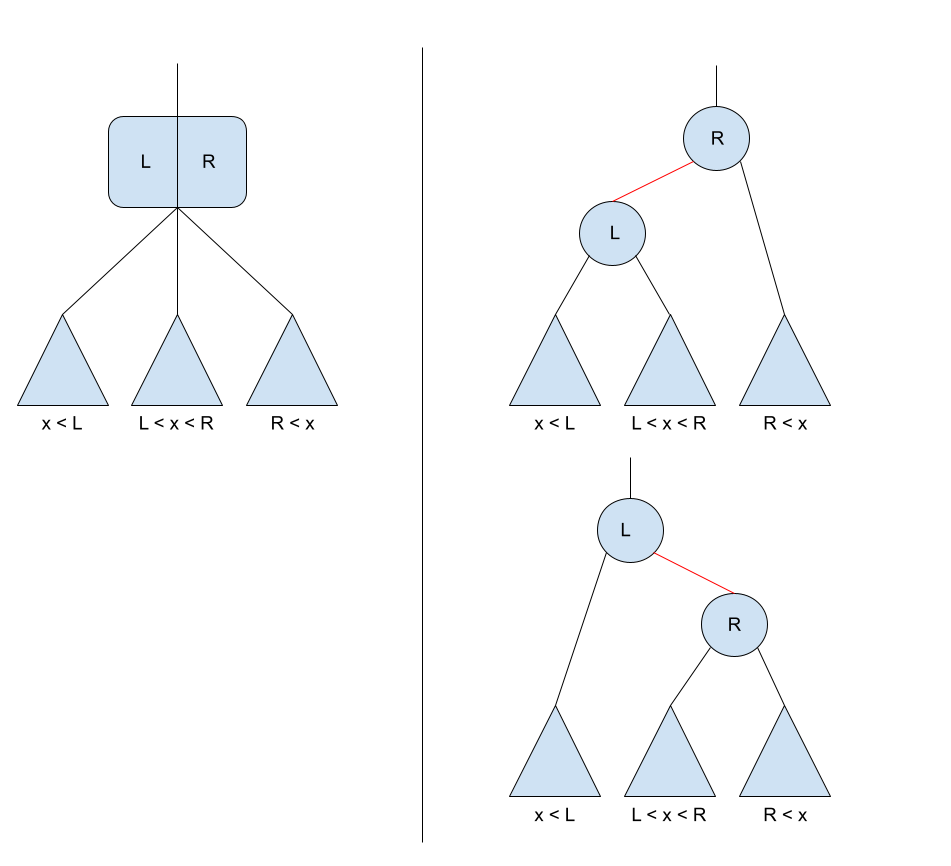
\includegraphics[width=0.65\textwidth]{rb_tree_1} \\
    A 3-node and its possible red-black tree versions. \\
    \vskip 1cm
\end{center}

    Since the height of a red-black tree is the number of black
    links the root must follow to get to a leaf, the two
    possible red-black subtrees above both have a height of $1$:
    the same height as the 2-3-4 tree they came from.

    The only remaining case is the 4-node. A 4-node usually only
    exists in a 2-3-4 tree for a moment before it is split
    apart. If we designate the $3$ items within the node as
    $a$, $b$, and $c$, then we say that (from left to right) the
    child links represent the ranges $x < a$, $a < x < b$,
    $b < x < c$, and $c < x$ for any item $x$ in the given
    child subtree. These cases, of course, can also be covered
    by an equivalent red-black tree, as shown below.

\begin{center}
    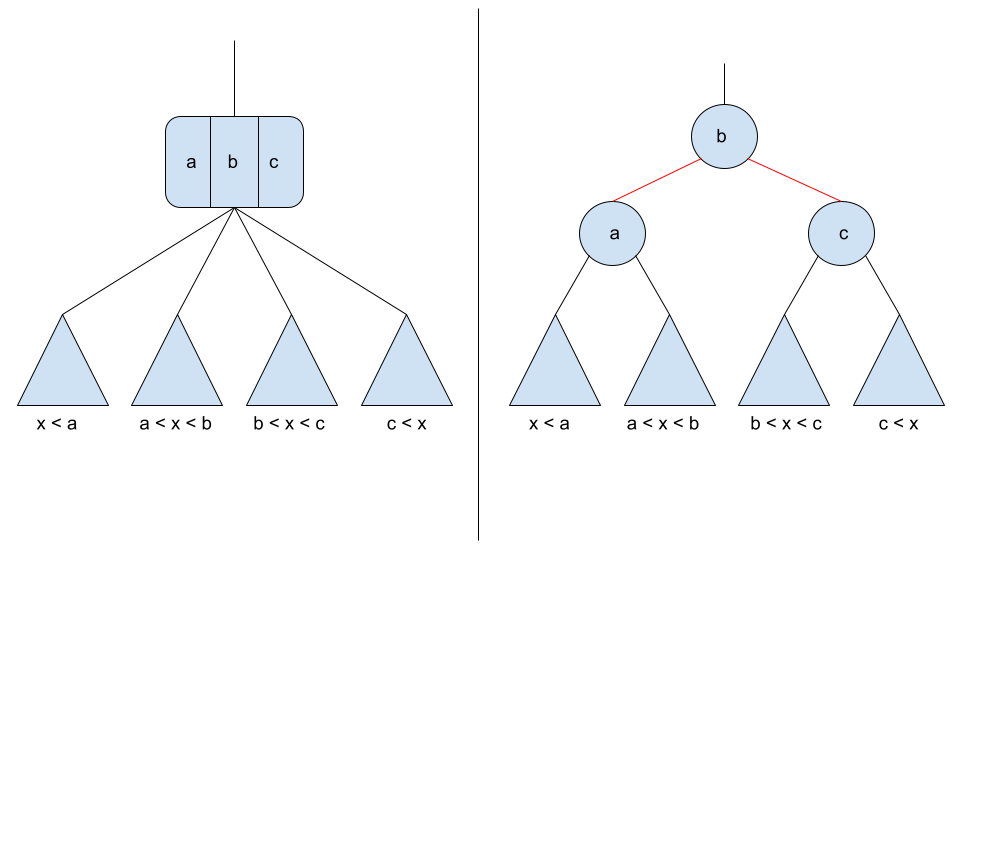
\includegraphics[width=0.65\textwidth]{rb_tree_2} \\
    A 4-node and its red-black tree version. \\
    \vskip 1cm
\end{center}

    Again, this red-black tree has the same height as its 2-3-4
    tree equivalent: $1$. Since we have accounted for all
    possible variations of red-black subtree herein, we can use
    the above rules to translate between red-black trees and
    2-3-4 trees. Therefore, any statement we make about 2-3-4
    trees holds for red-black trees.

    In the best-case scenario, a 2-3-4 tree (post 4-node
    splitting) containing $n$ nodes will have a height of
    $log_3(n)$, where every node is a 3-node. At worst case, it
    will have a height of $log_2(n)$, where every node is a
    2-node. Since red-black and 2-3-4 trees are equivalent, we
    can thusly say that the worst-case height of a red-black
    tree of size $n$ is limited by $log_2(n)$ black links.

    \newpage
    \textbf{Discuss how Red-Black trees are used in modern
    databases and file systems to maintain balanced structures.
    Explain the trade-offs and advantages of using Red-Black
    trees in these contexts.}

    To begin with, I will discuss the use of Red-Black trees in modern databases.
    Firstly, Red-Black trees provide efficient search and retrieval operations with a time complexity of O(log n). This makes them well-suited for databases, where quick access to data is crucial.
    
    Also, the self-balancing property of Red-Black trees ensures that it remains balanced during insertions and deletions. This property is vital in databases, because obtaining an asymmetric data structure can result in degraded performances.
    
    Finally, Red-Black trees are useful for querying a single or range elements, essential operation for a database.
    
    
    Red-Black trees are also very useful in file systems.
    Since they are capable of indexing and maintaining the hierarchical structure of directories in file systems, they permit to efficiently search for files.
    
    Also, as files are added or removed, the Red-Black tree's self-balancing property ensures that the directory structure remains balanced. This is important for maintaining quick and consistent file operations, such as searches and deletions.
    
    
    In these two contexts, their are some advantages and trade-off of using Red-Black trees.
    Red-Black trees guarantee a balanced structure, which results in predictable and efficient performance for various operations, including search, insertion, and deletion.
    
    Also, the worst-case time complexity for operations on Red-Black trees is O(log n), providing predictable and consistent performance in a variety of scenarios.
    
    Anyway, Red-Black trees require additional space to store color information for each node, which can increase the overall space overhead compared to simpler data structures.
    
    Moreover, the algorithms for maintaining the Red-Black tree's properties during insertions and deletions are more complex than those for simpler binary search trees, which may lead to slightly slower operations.
    
    Ultimately, Red-Black trees are a good choice for modern databases and file systems, that require predictable performance. 
    Anyway, the decision to use Red-Black trees involves trade-offs, such as increased space overhead and algorithmic complexity.
    The appropriateness of Red-Black trees depends on the specific requirements and characteristics of the application or system.
    
\section{Max Flow Algorithms}

\subsection{Theoretical Analysis}

    We will begin by analyzing the time and space complexity
    of the \textbf{Ford-Fulkerson algorithm} for max flow, and
    use this to motivate the segue into the Edmonds-Karp
    algorithm.

    The Ford-Fulkerson algorithm works by repeatedly finding an
    augmenting path (a path which can traverse the graph from
    the source node to the sink node and contains some amount of
    unused capacity) and adding the minimal flow across this
    path to the flow of each edge within. When no such path can
    be found, the graph has reached its maximal flow, and an
    answer to the problem can be returned. The pseudocode for
    the Ford-Fulkerson algorithm is shown below.

\begin{verbatim}
// 1) Initialize
Set all edges in flow graph to zero
Set residual graph to input graph

// 2) Iterate
While an augmenting path exists:
    Get augmenting path
    Add augmenting path to flow graph
    Subtract augmenting path from residual graph
End while

// 3) Output
Set net flow to zero
For edge exiting source node:
    Increment net flow by edge flow
End for

Return net flow
\end{verbatim}

    The most ambiguous part of this process is
    \verb|get augmenting path|. This vagueness has lead some to
    classify this process the Ford-Fulkerson method, rather than
    algorithm, as the time complexity could be vastly changed by
    the specific implementation of this line. For clarity, we
    will continue to refer to it as an algorithm. In our
    implementation, we will simply interpret this line to mean
    "choose the first augmenting path"- more specifically, 
    "at each node, if multiple augmenting paths are present,
    choose the one leading to the lowest-indexed node from this
    point". That is to say, if the paths \verb|0 -> 1 -> 2| and
    \verb|0 -> 3 -> 2| both exists, our initial algorithm would
    choose the first.

    Using these definitions and the above pseudocode, we can
    begin algorithmic analyses of the algorithm. We will call
    the set of all vertices $\mathbb{V}$, and the number of
    vertices $\vert \mathbb{V} \vert$. Similarly, the set of all
    edges and the number thereof are $\mathbb{E}$ and
    $\vert \mathbb{E} \vert$, respectively.
    
    The algorithm starts by initializing its variables, marked
    section 1 in the above code. These operations take
    $\vert \mathbb{E} \vert$ each. Next, the algorithm iterates
    over the augmenting paths. For each iteration, it gets an
    augmenting path, adds the augmenting path to the flow, and
    subtracts it from the residual. This means that this section
    runs with time proportional to the number of augmenting
    paths times two times the length of the current path. Each
    pass of this iteration is guaranteed to add at least 1 unit
    to the net flow, so there will be at most $f^*$ iterations,
    where $f^*$ is the maximal flow. The final section of the
    algorithm (section 3, which computes the calculated net
    flow), runs in time proportional to the number of edges
    leading from the source node, which is at most
    $\vert \mathbb{E} \vert$.

    Tying everything together, we can say that the
    Ford-Fulkerson algorithm runs in time proportional to

\[
    2 \cdot \vert \mathbb{E} \vert + f^* \cdot \vert \mathbb{E} \vert + \vert \mathbb{E} \vert
\]

    Converting this to big-O notation, we find that the running
    time complexity of the Ford-Fulkerson algorithm as listed
    here is $O(f^* \vert \mathbb{E} \vert )$.

    As written here, the Ford-Fulkerson algorithm uses several
    auxiliary variables of equal size to the input graph.
    However, were the preservation of the input graph not
    necessary, the operations using these variables could easily
    be modified to work by modifying the input graph. This
    means that, under proper optimization, the Ford-Fulkerson
    algorithm runs with space complexity $O(1)$.

    Having now finished analyzing the Ford-Fulkerson algorithm,
    we can move on to the Edmonds-Karp algorithm. As proven
    above, the Ford-Fulkerson algorithm can only be proved to
    converge upon the solution in time proportional to the max
    flow value itself. Thus, it is particularly unsuited for
    graphs with large maximal flows. Additionally, the original
    specification for the Ford-Fulkerson algorithm left the
    specific method used to select the next augmenting path
    unspecified. The solution to both of these problems comes
    in the form of the \textbf{Edmonds-Karp algorithm}.

    The Edmonds-Karp algorithm is a specific implementation of
    the Ford-Fulkerson method / algorithm wherein the next
    augmenting path to be chosen is the shortest one. This
    shortest path is chosen via breadth-first-search of the
    network. This allows the time complexity of the algorithm
    to become independent from $f*$. More specifically, the
    Edmonds-Karp algorithm runs in time complexity
    $O(\vert \mathbb{V} \vert \vert \mathbb{E} \vert ^2)$.

    The pseudocode for the Edmonds-Karp algorithm is listed
    below.

\begin{verbatim}
// 1) Initialize
Set all edges in flow graph to zero
Set residual graph to input graph

// 2) Iterate
While an augmenting path exists:
    Get shortest augmenting path via BFS
    Add augmenting path to flow graph
    Subtract augmenting path from residual graph
End while

// 3) Output
Set net flow to zero
For edge exiting source node:
    Increment net flow by edge flow
End for

Return net flow
\end{verbatim}

    Both algorithms as described here create copies of their
    input graphs for the flow and residual graphs. Additionally,
    neither the Ford-Fulkerson nor the Edmonds-Karp method of
    augmenting path discovery requires space larger than the
    size of the input graph. Thus, we can say that both
    algorithms run with space complexity bounded by the size of
    the input graph. Expressed in big-O notation, this appears
    as follows:

    \[
        O( \vert \mathbb{E} \vert + \vert \mathbb{V} \vert )
    \]

\subsection{Practical Implementation Details}

    The pseudocode from the previous section is fairly easy to
    translate into a viable program. However, we must first
    define how we will represent a weighted graph.

    We will represent a graph via a \verb|C++| vector of graph
    nodes. In turn, we will represent a graph node as a struct
    containing a \verb|C++| map mapping a node index to the
    weight on the edge associated with it. Additionally, a graph
    node will have a list of nodes which have edges pointing to
    it.

    We will represent an augmenting path as a vector of pairs of
    integers, with the first item being the index of the next
    node to visit and the second integer being the weight on
    that edge. For this representation to work, we also need to
    keep track of the initial node. We will use the same type
    graph data structure to represent the flow graph, the
    capacity graph, and the residual graph. To load graphs, we
    will use edge lists. Specifically, we will have the number
    of nodes, followed by the number of edges. After this, each
    edge will be three integers: The source node, the
    destination node, and the weight.

\begin{center}
    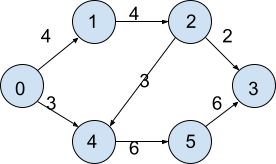
\includegraphics[width=0.4\textwidth]{graph} \\
    A benchmark graph for max-flow. \\
    \vskip 1cm
\end{center}

    Represented as an edge list, this graph would look like
    this:

\begin{verbatim}
    6 7
    0 1 4
    0 4 3
    1 2 4
    4 5 6
    2 4 3
    2 3 2
    5 3 6
\end{verbatim}

    Next, let's formalize the process by which we select
    augmenting paths for both algorithms. In the Ford-Fulkerson
    algorithm, we will use the following method.

\begin{verbatim}
Function to find the first augmenting path
Takes: The residual graph, start node, and sink node
Returns: The first augmenting path

    Let current = start node
    Let path = empty list
    Let visited = empty set

    While current != end node, do
        Insert current into visited

        For edge leading from current in order:
            If edge destination is in visited
                Continue
            End if

            If edge has additional flow remaining:
                Append edge onto path
                Current = edge destination
                Break from for loop
            End if
        End for
    End while

    Return path

End function

\end{verbatim}

    This returns the first available path, regardless of its
    length. Similarly, the Edmonds-Karp algorithm uses the
    pseudocode below to find the shortest available augmenting
    path.

\begin{verbatim}
Function to find the shortest augmenting path via BFS
Takes: The residual graph, start node, and sink node
Returns: The shortest augmenting path

    Let to_visit = queue
    Let came_from = array of size count(nodes) filled with -1

    push source node onto to_visit

    // Breadth-First Search

    While to_visit is not empty, do
        Let current = front of to_visit
        Pop front off of to_visit
        Insert current into visited

        For edge leading from current:
            If came_from[edge destination] == -1:
                came_from[edge destination] = current
                push edge destination onto to_visit

                If edge destination is sink node:
                    Break from for loop
                End if
            End if
        End for
    End while

    // Reconstruct path

    Let path = empty list
    Let current = sink node

    While current != source node, do
        If came_from[current] == -1:
            Return empty path
        End if

        Insert edge from came_from[current] to current at front of path
    End while

    Return path

End function

\end{verbatim}

    These two pseudocode functions complete our algorithm for
    the Ford-Fulkerson and the Edmonds-Karp algorithm. The
    \verb|C++| used in this project is a translation of this.

\subsection{Real-World Application}

    % TODO

\subsection{Theoretical Questions}

    \textbf{Describe the concept of augmenting paths and
    their role in the Ford-Fulkerson algorithm. Prove that the
    algorithm terminates and converges to the maximum flow in
    finite time, even for non-integer capacities.}

    An augmenting path is a path through the graph from the
    source node to the sink node such that a certain non-zero
    amount of flow may be added to the net flow between these
    nodes. An augmenting path is found in relation to a residual
    graph, which is a graph representing the remaining possible
    flow for each edge in the capacity graph. The residual graph
    is initialized as the capacity graph, and each additional
    augmenting path decreases the remaining flow in the residual
    graph by its net flow.

    The net flow across an augmenting path is defined as the
    smallest residual in any edge along that path.

    It is important to note that the net flow across the graph
    increases monotonically as a function of number of passes-
    That is to say that, for each additional augmenting path,
    the net flow must increase. In fact, the terminal condition
    of the algorithm is only met when no augmenting path with a
    net flow above zero can be found. Thus, any failure of this
    condition will result in the algorithm halting.

    Let us assume the following:
    \begin{itemize}
        \item With zero augmenting paths, the net flow is zero
        \item An augmenting path must increase the net flow
        \item The net flow is a finite real number greater than
            or equal to zero
        \item The net flow is equal to the sum of the net flows
            of the augmenting paths
    \end{itemize}

    Mathematically:
    \[
    \begin{aligned}
        p \in \mathbb{R}^n , &\left[ \forall p_i \in p \right] p_i > 0 \\
        f^* \in \mathbb{R}: 0 &\le f^* < \infty \\
        \sum_{i = 0}^n { p_i } &= f^* \\
        &\therefore \\
        \sum_{i = 0}^n p_i < \infty , &\left[ \forall p_i \in p \right] p_i > 0 \\
        &\therefore \\
        n &< \infty \\
    \end{aligned}
    \]

    That is to say, that since the net flow is a sum of non-zero
    real numbers and it is itself a finite real number, it must
    be a finite sum. This implies that the number of augmenting
    paths must be finite, implying that the algorithm converges
    in finite time.

    Since we only assumed that the net flow across an augmenting
    path is a real number, this proves the convergence of this
    method upon both integer and non-integer weights.

    \textbf{Explain the Min-Cut Max-Flow Theorem and its
    significance in the context of network flows. How can this
    theorem be used to find a maximum flow and minimum cut in a
    flow network?}

    % TODO - Jordan

    The Min-Cut Max-Flow Theorem states that the cost of the
    min-cut across a network is the same as the maximal flow
    across that network.

    Since we have just defined several algorithms for finding
    the max flow across a network, the theorem allows us to also
    use these algorithms to find the minimum cut.

\section{Real-World Problem Solving}

    % TODO

\section{Comparative Analysis and Reporting}

\subsection{Red-Black Trees}

    % TODO

\subsection{Max Flow Algorithms}
    Below is a graph of running times from a series of
    experimental runs of the Ford-Fulkerson (FF) and
    Edmonds-Karp (EK) algorithms on various randomly-generated
    graphs.

\begin{center}
    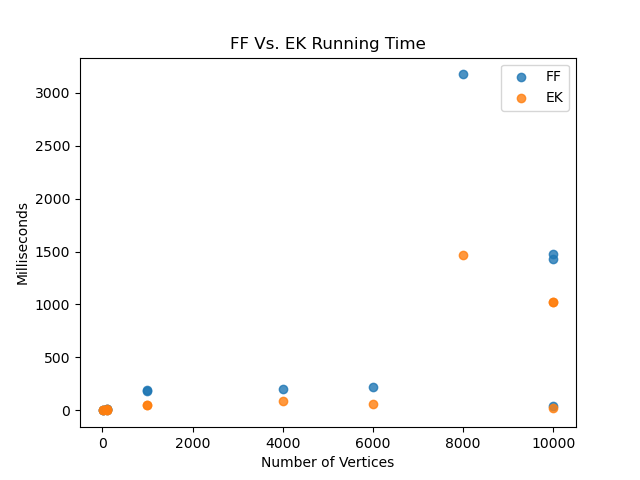
\includegraphics[width=0.65\textwidth]{mf_algorithm_comparison} \\
    The Ford-Fulkerson (FF) algorithm vs the Edmonds-Karp (EK)
    algorithm on randomly generated graphs of various size. \\
    \vskip 1cm
\end{center}

    Clearly, the Edmonds-Karp algorithm performs reliably
    better than the original Ford-Fulkerson one, especially for
    large graphs.

    The below graph shows the number of augmenting paths present
    in graphs of various sizes.

\begin{center}
    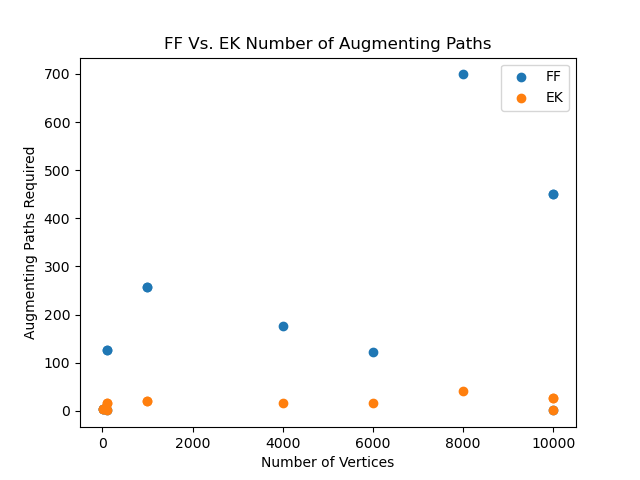
\includegraphics[width=0.65\textwidth]{mf_passes_comparison.png} \\
    The Ford-Fulkerson (FF) algorithm vs the Edmonds-Karp (EK)
    algorithm on various graphs, by number of passes required. \\
    \vskip 1cm
\end{center}

    Although the difference is not always extreme, the
    Edmonds-Karp algorithm reliably runs at worst as well as
    Ford-Fulkerson, and usually much better. From this data, it
    would seem that EK is the best choice. However, this is not
    always the case.

\begin{verbatim}
In a graph w/ 1000 nodes and 631216 edges
1 <= weight <= 10

FF ms:     22,950.6
FF passes: 2,732

EK ms:     151,082.0
EK passes: 1,243

\end{verbatim}

    The above output exemplifies a case in which the
    Ford-Fulkerson algorithm outperforms the Edmonds-Karp one.
    Here, EK ran in 151 seconds, while FF took only 23 seconds.
    This is because of the disparity between $f^*$ (3,161),
    $\vert \mathbb{E} \vert$ (631,216), and
    $\vert \mathbb{V} \vert$ (1,000). Since FF runs in time
    proportional to $f^* \cdot \vert \mathbb{E} \vert$, we can
    expect it to run in approximately
    $3,161 \cdot 631,216 = 1,995,273,776$ operations. EK, on the
    other hand, will run in about
    $1,000 \cdot 631,216^2 = 398,433,638,656,000$ operations-
    $5$ orders of magnitude more! Luckily, EK only performed $1$
    order of magnitude worse than FF in our experiment, but this
    is still a non-trivial performance cost in what is supposed
    to be the better algorithm.

    Thus, the choice between FF and EK is more nuanced than it
    first would seem.

\section{Conclusion}

\subsection{Red-Black Trees}
    
    % TODO

\subsection{Maxflow}

    The EK algorithm was developed as an instance of the FF
    algorithm, specifically optimized to remove FF's complexity
    reliance upon $f^*$. Thus, in cases where $f^*$ is very
    large in comparison to $\vert \mathbb{E} \vert$ and
    $\vert \mathbb{V} \vert$, EK will be the more efficient
    choice. It will require fewer augmenting paths, and each
    augmenting path will increase the total flow more. However,
    each of these augmenting paths will be more costly to
    compute. Thus, if $f^*$ is very small in comparison to the
    number of nodes and edges, FF will run more efficiently.

    It is notable that, even in the failure case described
    above, EK will still require fewer augmenting paths than FF.
    It is simply the cost of computing these paths which causes
    EK to fail.

    Since it is rare that $f^* \cdot \vert \mathbb{E} \vert$ is
    smaller than
    $\vert \mathbb{V} \vert \vert \mathbb{E} \vert ^2$, EK will
    most often be the correct choice for the maxflow problem.
    However, the wisest approach would be to implement both
    algorithms, and switch to FF if it is computed to be more
    efficient.

\newpage
\section{References}

\begin{verbatim}
[1] "2-3-4 Trees and Red- Black Trees.” Purdue University,
        www.cs.purdue.edu/homes/ayg/CS251/slides/chap13b.pdf.
        Accessed 28 Nov. 2023. 

[2] "Edmonds-Karp Algorithm.” Brilliant Math; Science Wiki,
        brilliant.org/wiki/edmonds-karp-algorithm/. Accessed 28
        Nov. 2023. 

[3] "Ford-Fulkerson Algorithm for Maximum Flow Problem.”
        GeeksforGeeks, GeeksforGeeks, 1 June 2023,
        www.geeksforgeeks.org/ford-fulkerson-algorithm-for-maximum-flow-problem/. 

[4] "Ford-Fulkerson Algorithm.” Brilliant Math; Science Wiki,
        brilliant.org/wiki/ford-fulkerson-algorithm/. Accessed 28
        Nov. 2023. 

[5] Sedgewick, Robert. Left-Leaning Red-Black Trees,
        sedgewick.io/wp-content/themes/sedgewick/papers/2008LLRB.pdf.
        Accessed 28 Nov. 2023. 
\end{verbatim}

\end{document}
